\newpage
\section{Début du travail, d'un point de vue théorique et/ou numérique}

\vspace{0.6cm}

Pour commencer notre projet, on a tout d'abord effectué des recherches documentaires sur différents termes pour en apprendre davantage sur le mode de  fonctionnement de notre interface de jeu tel que : \
\begin{itemize}
    \item[$\bullet$] la programmation dynamique ;
    \item[$\bullet$] l'apprentissage par renforcement ;
    \item [$\bullet$]l'environnement stochastique ;
    \item[$\bullet$] le model based / model free ;
    \item[$\bullet$] processus décisionnel Markovien.


\end{itemize}
\vspace{0,5cm}

Par la suite, on a commencé à traiter notre projet théoriquement. En effet, ce projet comme expliqué précédemment consiste à créer un code qui permet à notre agent de se déplacer dans un environnement grâce à des actions (aller en bas, à gauche, à droite, en haut) et à chaque déplacement, l'agent perdra un point sur son score et en fonction de la case où il va pourra gagner ou perdre des points (+100 points pour les donuts et -100 points pour des cases avec un ennemi).
Puis, afin de réaliser un environnement, on a commencé à l'imaginer en essayant de créer une grille dans laquelle on placera nos agents et, concernant les actions ces dernières font intervenir la notion de probabilité puisque l'agent pour se tromper lorsqu'on lui indiquera le chemin à suivre. Suite à cela, nous avons calculé une matrice de corrélation sur un modèle simple et petit afin de la mettre en oeuvre pour un modèle plus complexe.  \\

D'un point de vue numérique, on a reçu un code implémenté de la part de notre encadrante pour avoir l'interface du jeu et des mouvements d'un agent, et cela afin d'avoir un aperçu du fonctionnement du jeu et également s'inspirer de quelques idées. Maintenant, à partir de ce qu'on a étudié et reçu par notre encadrante, nous allons reprendre le jeu et mettre en place un système d'apprentissage pour que l'agent apprenne et finisse par trouver le chemin qui maximise son score.

\vspace{0.7cm}

\FloatBarrier %bloque l'image dans le texte
\begin{figure}[!h]
\centering
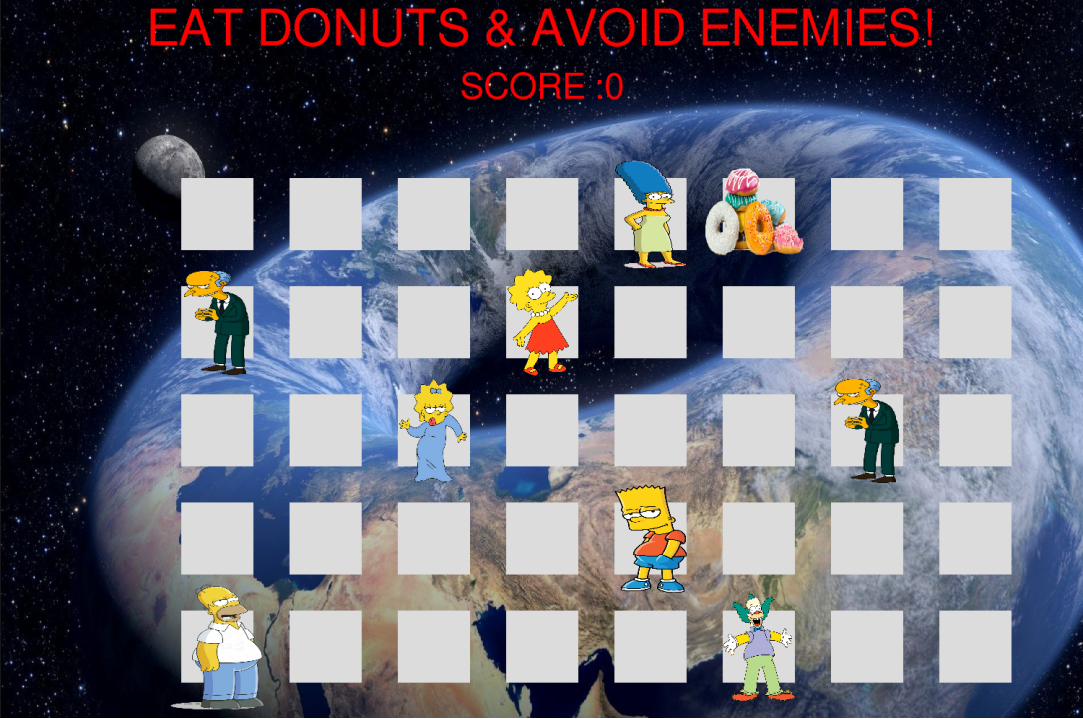
\includegraphics[width=14cm,scale=1]{Capture.PNG}
\caption{Interface obtenue}
\end{figure}
\FloatBarrier